\BourbakiBackSection{历史注记}

（括号中的数字指本注记末尾的参考文献。）

极限与连续的观念可以追溯到古代；若不从这个观点出发，不仅对希腊数学家、而且对希腊哲学家、特别是亚里士多德进行系统的研究，就无法写出一部完整的极限与连续观念史。此外，还必须追溯这些观念在文艺复兴时期数学中以及 在微分学与积分学开端时期的演变。这样一项研究，尽管进行起来无疑会引人入胜，却将远远超出本注记的范围。

应当认为是 Riemann 创立了拓扑学，正如现代数学的许多其他分支一样。他第一个尝试表述拓扑空间的概念；他孕育了关于这种空间的自足理论的设想；他定义了在拓扑学后来的发展中起卓越作用的不变量（“Betti 数”）；他第一个把拓扑学应用于分析（Abel 积分的周期）。但是，十九世纪上半叶的思想潮流已经从不止一个方面为 Riemann 铺平了道路。首先，把数学建立在坚实基础之上的愿望——它是整个十九世纪直至今天许多重要研究的缘由——使人们正确理解了收敛级数与趋于极限的数列的概念（Cauchy、Abel），以及连续函数的概念（Bolzano、Cauchy）。另一方面，由 Gauss 与 Argand 提出的复数（或者像以前人们所称的那样，“虚”数甚至“不可能”数）的几何表示（以平面上的点表示），已为大多数数学家所熟悉；这一进步与本世纪在 Hilbert 空间研究中采用几何语言具有同一数量级，并且蕴含着对每个能连续变化的对象进行几何表示这一可能性的萌芽。至于 Gauss，他本来就会由于其关于几何基础、非欧几何与曲面的研究而自然地达到这类概念，而且他似乎早已想到这种可能性，因为他在（独立于 Argand 与法国数学家）定义复数的几何表示时使用了“二次延展的量”一语（{[}1{]}，第 101-103 页及第 175-178 页）。

Riemann 关于代数函数及其积分的工作，以及他对几何基础的思考（在很大程度上来自他对 Gauss 著作的研究），使他制定了一个研究纲领，这恰好就是现代拓扑学的纲领，并使他开始实现这一纲领。例如，他在其 Abel 函数论中说道（{[}2{]}，第 91 页）：

“在研究由恰当微分的积分所得到的函数时，Analysis situs 的某些定理几乎是不可或缺的。这个由 Leibnitz 用过的名称（尽管也许是在多少有些不同的意义上）应当称呼连续量理论中这样的部分：它研究这些量时，不是脱离它们的位置、以它们彼此度量来研究，而是撇开一切度量观念，只考虑它们的位置关系与包含关系。我把它完全脱离一切度量的研究留给以后的机会\ldots{}”

而在其著名的就职演说“论几何学所赖以成立的假设”（{[}2{]}，第 272 页）中：

“\ldots{} 多次延展的量的一般概念（(*)）——它把空间量概念作为特例包含在内——至今完全没有得到研究\ldots”（第 272 页）

“\ldots{} 量的概念以一个元素可作各种不同的规定为前提。按照能否经由连续的过渡过程从一个规定过渡到另一个规定，这些规定构成一个连续流形或一个离散流形：在前一情形，这些规定称为该流形的点\ldots”（第 273 页）

“\ldots{} 度量在于把待比较的量叠合起来，因此为了度量，我们需要某种以一个量作为另一个量的尺度的手段。缺乏这种手段时，只有当一个量是另一个量的一部分时，我们才能比较这两个量\ldots{} 在此情形下所能进行的研究构成量理论中独立于度量理论的一部分，其中诸量不被看作独立于其位置而存在，也不被看作可用度量单位表出，而是被看作流形中的区域。这样的研究在数学的若干部分中已成为必要，特别是在多值解析函数论中\ldots”（第 274 页）

“\ldots{} 在给定的流形中，只要这是可能的，位置的确定都可归结为有限多个数值规定。然而存在这样的流形，其中位置的确定需要的不是有限多个规定，而是一个无穷序列、甚至是量规定的一个连续流形。例如，一个函数在给定区域上的各种可能规定，或者一个空间图形的各种可能形状，都给出这种类型的流形。”（第 276 页）

请注意最后这段话中函数空间研究的最初观念；Riemann 在其博士论文中已经表述过同一观念：他在谈到被称为 Dirichlet 原理的极小问题时说道，“这些函数的全体”“构成一个自身封闭的连通区域”（{[}2{]}，第 30 页）；这一表述虽不完善，却正是 Hilbert 后来给出的 Dirichlet 原理的证明、以及函数空间对变分法的大部分应用的萌芽。

如前所述，Riemann 开始实施这一宏伟纲领：他定义了“Betti 数”，先是对曲面（{[}2{]}，第 92-93 页），后来（{[}2{]}，第 479-482 页；另参看{[}3{]}）对任意维数的流形，并把这一定义应用于积分论；关于这一点以及这一理论自 Riemann 时代以来的巨大发展，请读者参看本丛书中代数拓扑各章的历史注记。

在 Riemann 所设想的那种拓扑空间的一般理论得以发展之前，实数理论、数集理论以及直线上、平面上与空间中的点集理论，都必须比 Riemann 时代得到更为系统的研究。这些研究另一方面与关于无理数本性的探讨（Bolzano 的半哲学式探讨与 Dedekind 的本质上数学的探讨）以及实变函数论中的进展相联系；在实变函数论中，Riemann 本人以其积分定义与其三角级数理论作出了重要贡献，du Bois-Reymond、Dini 与 Weierstrass 等人也对它有所贡献；这些工作是十九世纪下半叶的工作，尤其是 Cantor 的工作，他第一个（最初在直线上，后来在 n 维欧氏空间中）定义了聚点、闭集、开集、完备集诸概念，并得到了关于这些集合在直线上的结构的主要结果（参看第四章的历史注记）。在这方面，不仅应参看 Cantor 的著作{[}4{]}，还应参看他与 Dedekind 的极其有趣的通信{[}5{]}，其中可以找到维数作为拓扑不变量这一思想的明确表述。该理论后来的进展在 Schoenflies 的书{[}6{]}中以半历史、半系统的方式加以追溯；迄今最重要的收获是 Borel-Lebesgue 定理，即欧氏 \(n\) 维空间 \(\mathbf{R}^n\)（参看第六章，§ 1）的每个有界闭子集都满足本章 § 9 的公理（C \(^{''}\)）这一事实（该定理最初是 Borel 对直线上的一个闭区间以及覆盖它的可数开区间族证明的）。

Cantor 的思想最初曾遭到激烈的反对（参看第一卷第一章至第四章的历史注记）。无论如何，他关于直线上与平面上的点集的理论很快就被法国与德国的函数论学派（Jordan、Poincaré、Klein、Mittag-Leffler，以及后来的 Hadamard、Borel、Baire、Lebesgue 等）所利用和传播；特别是 Borel 早期的每部教程都含有这一理论的初等阐述（例如见{[}7{]}）。随着这些思想的传播，把它们应用于不是由点组成、而是由曲线或函数组成的集合的可能性，开始在各个方面被考虑，其见证是 Ascoli 1883 年一篇论文的标题“论一簇曲线的极限曲线”{[}8{]}，以及 Hadamard 1896 年在苏黎世数学家大会上的报告{[}9{]}；所有这些都与 Volterra 1887 年引入“线函数”以及创立“泛函演算”即自变量为函数的函数论密切相关（参看 Volterra 关于泛函分析的书{[}10{]}）。另一方面，Hilbert 的著名论文{[}11{]}——他在其中重新采纳 Riemann 的思想，证明了 Dirichlet 原理中最小值的存在，并开创了变分法中的“直接方法”——清楚地表明了考虑使 Bolzano-Weierstrass 原理成立、也就是说使每个序列都有收敛子列的函数集的重要性。这类集合无论如何已开始起重要作用，不仅在变分法中，而且在实变函数论中（Ascoli、Arzelà），稍后还在复变函数论中（Vitali、Carathéodory、Montel）。最后，函数方程的研究、特别是 Fredholm 对冠以其名的那类方程的求解，使把函数看作变元、把函数集看作点集成为常见之事，并且使在这一场合使用几何语言如同在 \(n\) 维欧氏空间中一样自然（这种空间同样逃避“直观”，因此长期是许多数学家不信任的对象）。特别是 Hilbert 关于积分方程的值得纪念的工作{[}12{]}导致 Erhard Schmidt{[}14{]}对 Hilbert 空间的定义与几何研究，与欧氏几何完全类似。

与此同时，公理理论的概念由于几何基础方面的大量工作而变得越来越重要；在这方面，Hilbert 的贡献{[}13{]}具有特别决定性的影响。在这项工作过程中，Hilbert 于 1902 年（{[}13{]}，第 180 页）给出了 Riemann 意义下“二次延展流形”的第一个公理化定义，Hilbert 说这个定义构成“对 Analysis situs 作严格公理处理的基石”。Hilbert 还使用了邻域（其意义受他把自己局限于其中的问题的要求的限制）。

把点集性质与函数集性质的共同内容抽象出来的最初尝试应归功于 Fréchet{[}15{]}与 F. Riesz{[}16{]}。前者从可数极限的概念出发，未能构造出一个方便而富有成效的公理系统，但至少他认识到了 Bolzano-Weierstrass 原理{[}即 § 9 的公理（C）限于可数序列的情形{]}与 Borel-Lebesgue 定理{[}§ 9 的公理（C''）{]}之间的关系；正是在这一场合他引入了“紧”这个词，尽管其意义与本丛书所用者略有不同。至于 F. Riesz，他以聚点概念（或者不如说“导集”概念，这二者是一回事）为出发点，他的理论仍不完全，且只以概要的形式出现。

今天所理解的一般拓扑学始于 Hausdorff（{[}17{]}，第 7、8、9 章），他重新采用了邻域概念（他所谓邻域，即本丛书术语中所称的“开邻域”），并从 Hilbert 关于平面上邻域的公理中挑选出那些能使其理论具有所期望的全部精确性与一般性的公理。他作为出发点的公理本质上是（考虑到他的邻域概念与我们的邻域概念之间的差别）§ I 的公理（ \(V_{I}\)）、（ \(V_{II}\)）、（ \(V_{III}\)）、（ \(V_{IV}\)）以及 § 8 的（H），而他推演这些公理的推论的那一章一直是公理理论的一个典范：抽象而又预先适应于应用。Hausdorff 的工作自然是后来一般拓扑学研究、特别是莫斯科学派工作的出发点，后者的工作大部分指向度量化问题（参看第九章的历史注记）；这里我们特别回顾 Alexandroff 与 Urysohn 对紧空间的定义（以“双紧空间”之名），以及 Tychonoff 关于紧空间的积仍为紧空间的证明{[}19{]}。最后，H. Cartan{[}20{]}引入滤子给拓扑学带来了一件宝贵的工具，可用于各种各样的应用（在其中它比“Moore-Smith 收敛”概念{[}18{]}更为有利）。此外，超滤子定理（定理 1，§ 6）的发展阐明并简化了理论。

\BourbakiBackSection{参考文献}

{[}1{]} C. F. GAUSS, Werke, Vol. 2, Göttingen, 1863.

{[}2{]} B. RIEMANN, Gesammelte mathematische Werke, 2nd edition, Leipzig (Teubner), 1892.

{[}3{]} B. RIEMANN, in Lettere di E. Betti a P. Tardy, Rend. Accad. Lincei (5) 24 \(^{1}\) (1915) pp.~517-519.

{[}4{]} G. CANTOR, Gesammelte Abhandlungen, Berlin (Springer), 1932.

{[}5{]} G. CANTOR and R. DEDEKIND, Briefwechsel, Actualités scientifiques et industrielles, no. 518, Paris (Hermann), 1937.

{[}6{]} A. SCHOENFLIES, Entwicklungen der Mengenlehre und ihrer Anwendungen, Part I, 2nd edition, Leipzig-Berlin (Teubner), 1913.

{[}7{]} E. BOREL, Leçons sur la théorie des fonctions, 2nd edition, Paris (Gauthier-Villars), 1914.

{[}8{]} G. Ascoli, Le curve limiti di una varietà data di curve, Mem. Accad. Lincei (3) 18 (1883) p.~521-586.

{[}9{]} J. HADAMARD, Sur certaines applications possibles de la théorie des ensembles, Verhandl. Intern. Math.-Kongress, Zürich, 1898, pp.~201-202.

{[}10{]} V. VOLTERRA, Theory of Functionals, London-Glasgow (Blackie and Son), 1930.

{[}11{]} D. HILBERT, Gesammelte Abhandlungen, vol.~3, Berlin (Springer), 1935, pp.~10-37 {[}= Jahresbericht des D.M.V., 8 (1900), p.~184, and Math. Ann., 59 (1904), p.~161{]}.

{[}12{]} D. HILBERT, Grundzüge einer allgemeinen Theorie der Integralgleichungen, 2nd edition, Leipzig-Berlin (Teubner), 1924.

{[}13{]} D. HILBERT, Grundlagen der Geometrie, 7th edition, Leipzig-Berlin (Teubner), 1930.

{[}14{]} E. SCHMIDT, Über die Auflösung linearer Gleichungen mit unendlich vielen Unbekannten, Rend. Palermo, 25 (1908), pp.~53-77.

{[}15{]} M. FRÉCHET, Sur quelques points du calcul fonctionnel, Rend. Palermo, 22 (1906), pp.~1-74.

{[}16{]} F. RIESZ, Stetigkeitsbegriff und abstrakte Mengenlehre, Atti del IV Congresso Intern. dei Matem., Bologna, 1908, vol.~2, pp.~18-24.

{[}17{]} F. HAUSDORFF, Grundzüge der Mengenlehre, 1st edition, Leipzig (Veit), 1914.

{[}18{]} E. H. MOORE and H. L. SMITH, A general theory of limits, Am. Journ. of Math., 44 (1922) pp.~102-121.

{[}19{]} A. TYCHONOFF, Über die topologische Erweiterung von Räumen, Math. Ann., 102 (1930), pp.~514-561.

{[}20{]} H. CARTAN, Théorie des filtres; filtres et ultrafiltres, C. R. Acad. Sc. Paris, 205 (1937), pp.~595-598 and pp.~777-779.

\chapter{一致结构}

\section{一致空间}

\subsection{一致结构的定义}

定义 1 集合 X 上的一致结构（或一致）是这样的结构：它由 X × X 的一个子集族 U 给出，该子集族满足第一章 § 6 第 1 目的公理（F\_I）与（F\_II），并且还满足下列公理：

\((\mathbf{U}_{\mathbf{I}})\) 属于 \(\mathfrak{U}\) 的每个集合都含对角线 \(\Delta\)。

\((\mathbf{U}_{\mathbf{II}})\) 若 \(\mathbf{V}\in \mathfrak{U}\)，则 \(\overline{\mathbf{V}}^1\in \mathfrak{U}\)。

\((\mathbf{U}_{\mathbf{III}})\) 对每个 \(\mathbf{V} \in \mathfrak{U}\)，存在 \(\mathbf{W} \in \mathfrak{U}\) 使 \(\mathbf{W} \circ \mathbf{W} \subset \mathbf{V}\)。

\pandocbounded{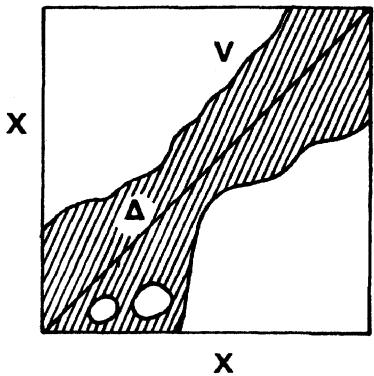
\includegraphics[keepaspectratio]{images/part001_6ce88dc6.jpg}}\\
图 2.

\(\mathfrak{U}\) 中的诸集合称为在 \(\mathbf{X}\) 上由 \(\mathfrak{U}\) 所定义的一致结构的一致邻域。赋有一致结构的集合称为一致空间。

若 V 是集合 X 上某个一致结构的一致邻域，我们可以把关系 \((x, x') \in V\) 表述为“x 与 \(x'\) 是 V-邻近的”。

注。1）为使语言更富表现力，我们可以在某些陈述中使用“x 与 y 足够接近”“x 与 y 要多接近就有多接近”这类说法。例如，我们将说，一个关系

R \(\{x,y\}\) 只要 x 与 y 足够接近便为真，如果存在一致邻域 V，使关系 \((x,y)\in V\) 蕴含 R \(\{x,y\}\)。

\begin{enumerate}
\def\labelenumi{\arabic{enumi})}
\setcounter{enumi}{1}
\tightlist
\item
  公理（U \(_{II}\)）与（U \(_{III}\)）的合取（在一致结构的其余公理之下）等价于下述公理：
\end{enumerate}

\((\mathbf{U}_a)\) 对每个 \(\mathbf{V} \in \mathfrak{U}\)，存在 \(\mathbf{W} \in \mathfrak{U}\) 使 \(\mathbf{W} \circ \overline{\mathbf{W}} \subset \mathbf{V}\) (*)。

显然 \((\mathbf{U}_{\mathrm{II}})\) 与 \((\mathbf{U}_{\mathrm{III}})\) 蕴含 \((\mathbf{U}_a)\)。反之，若 \((\mathbf{U}_a)\) 成立，我们有 \(\overline{\mathbf{W}} = \Delta \circ \overline{\mathbf{W}} \subset \mathbf{V}\)（由 \((\mathbf{U}_I)\)）；于是 \(\mathbf{W} \subset \overline{\mathbf{V}}\)，从而{[}由 \((\mathbf{F}_I)] \overline{\mathbf{V}} \in \mathfrak{U}\)。令 \(\mathbf{W}' = \mathbf{W} \cap \overline{\mathbf{W}}\)；则 \(\mathbf{W}' \in \mathfrak{U}\)（由刚才所证及公理 \((\mathbf{F}_{\mathrm{II}})\)），并且 \(\mathbf{W}' \circ \mathbf{W}' \subset \mathbf{W} \circ \overline{\mathbf{W}} \subset \mathbf{V}\)。

本章中我们始终用 \(\mathbf{V}\) 代替 \(\mathbf{V} \circ \mathbf{V}\)，一般地写 \(\mathbf{V} = \mathbf{V} \circ \mathbf{V} = \mathbf{V} \circ \mathbf{V}\)，其中 \(n > 1\) 为整数，\(\mathbf{V}\) 为 \(\mathbf{X} \times \mathbf{X}\) 的子集。

\begin{enumerate}
\def\labelenumi{\arabic{enumi})}
\setcounter{enumi}{2}
\tightlist
\item
  若 X 非空，则公理 \((U_{I})\) 蕴含 U 中没有一个集合是空集，从而 U 是 \(X \times X\) 上的一个滤子。空集上只有一个一致结构，即 \(U = \{\varnothing\}\)。
\end{enumerate}

定义 2 一致结构的一致邻域基本系是指由一致邻域组成的任一这样的族 B：每个一致邻域都含有属于 B 的一个集合。

公理 \((\mathbf{U}_{\mathbf{III}})\) 表明，若 n 为任一整数 \textgreater0 且 V 取遍某个一致邻域基本系，则诸集合 \(V^{n}\) 仍构成一个一致邻域基本系。

满足 \(V = \overline{V}^{1}\) 的一致邻域 V 称为对称的。若 V 是任一一致邻域，则 \(V \cap \overline{V}^{1}\) 与 \(V \cup \overline{V}^{1}\) 都是对称一致邻域，并且公理 \((F_{\mathrm{II}})\) 与 \((U_{\mathrm{II}})\) 表明诸对称一致邻域构成一个一致邻域基本系。

子集族 \(\mathfrak{B}\)——它由 \(\mathbf{X} \times \mathbf{X}\) 的子集组成——是 \(\mathbf{X}\) 上某个一致结构的一致邻域基本系，当且仅当 \(\mathfrak{B}\) 满足第一章 § 6 第 3 目的公理（ \(B_{\mathbf{I}}\)），并且还满足下列公理：

\((\mathbf{U}_{\mathbf{I}}^{\prime})\) \(\mathfrak{B}\) 中的每个集合都含对角线 \(\Delta\)。

\((\mathbf{U}_{\mathbf{II}}^{\prime})\) 对每个 \(\mathbf{V} \in \mathfrak{B}\)，存在 \(\mathbf{V}' \in \mathfrak{B}\) 使 \(\mathbf{V}' \subset \overline{\mathbf{V}}^1\)。

\((\mathbf{U}_{\mathbf{III}}^{\prime})\) 对每个 \(\mathbf{V} \in \mathfrak{B}\)，存在 \(\mathbf{W} \in \mathfrak{B}\) 使 \(\tilde{\mathbf{W}} \subset \mathbf{V}\)。

若 X 非空，则 X 上一致结构的一致邻域基本系是由该结构的诸一致邻域组成的滤子的一个基（第一章 § 6 第 3 目命题 3）。

(*) 我们回顾（《集合论》，R，§ 3，第 4 与第 10 目）：若 V 与 W 是 \(\mathbf{X} \times \mathbf{X}\) 的两个子集，则由对 \((x, y) \in \mathbf{X} \times \mathbf{X}\)（它们满足：\((x, z) \in \mathbf{W}\) 且 \((z, y) \in \mathbf{V}\) 对某个 \(z \in \mathbf{X}\) 成立）组成的集合记作 V o W 或 VW，而由对 \((x, y) \in \mathbf{X} \times \mathbf{X}\) 中满足 \((y, x) \in \mathbf{V}\) 者组成的集合记作 \(\overline{\mathbf{V}}\)。

一致结构的例子。* 1）在实数集 R 上可以如下定义一个称为加法一致结构的一致结构：对每个 \(\alpha > 0\)，令 \(V_{\alpha}\) 为 \(R \times R\) 中由对 \((x, y)\)（满足 \(|x - y| < \alpha\)）全体组成的子集；当 \(\alpha\) 取遍一切实数 \(> 0\) 时，诸 \(V_{\alpha}\) 构成 R 上加法一致结构的一个一致邻域基本系。类似地，在有理数集 Q 上可以定义一个一致结构（也称加法一致结构）；我们将在第三章与第四章中研究这些结构以及群上类似的一致结构。* 2）设 X 是一个集合，R 是 X 上的一个等价关系；令 C 为

R 在 \(\mathbf{X} \times \mathbf{X}\) 中的图像。于是 \(\Delta \subset \mathbf{C}\) 且 \(\tilde{\mathbf{C}} = \tilde{\mathbf{C}} = \mathbf{C}\)（《集合论》，R，§ 5，第 1 目）；因此由单独一个集合 C 组成的 \(\mathbf{X} \times \mathbf{X}\) 的子集族是 X 上某个一致结构的一致邻域基本系。特别地，若取 R 为相等关系，则 \(\mathbf{C} = \Delta\)，而相应一致结构的诸一致邻域是 \(\mathbf{X} \times \mathbf{X}\) 中含 \(\Delta\) 的一切子集；这个一致结构称为 X 上的离散一致结构，赋有这个一致结构的集合 X 称为离散一致空间。

\begin{enumerate}
\def\labelenumi{\arabic{enumi})}
\setcounter{enumi}{2}
\tightlist
\item
  在有理整数集 \(\mathbf{Z}\) 上可以如下定义一个在数论中重要的一致结构：给定一个素数 \(p\)，令 \(\mathbf{W}_n\) 为由对 \((x,y)\in \mathbf{Z}\times \mathbf{Z}\) 中满足 \(x\equiv y\)（mod \(p^n\)）者全体组成的集，这里 \(n > 0\) 为任意整数。容易验证，诸集合 \(\mathbf{W}_n\)（对固定的 \(p\)）构成 \(\mathbf{Z}\) 上某个一致结构的一致邻域基本系，该一致结构称为 \(p\) 进一致结构（参看第三章 § 6 习题 23 及以后，以及第九章 § 3 第 2 目）。
\end{enumerate}

按照一般的定义（《集合论》，R，§ 8，第 5 目），若 X 与 X' 是两个各赋有一致结构的集合，其一致邻域族分别为 U 与 U'，则 X 到 X' 上的双射 f 是 X 的一致结构到 X' 的一致结构上的同构，如果 g(U) = U'，其中 g = f × f。

例如，若 X 与 \(X'\) 是两个等势的集合，则 X 到 \(X'\) 上的每个双射都是 X 的离散一致结构到 \(X'\) 的离散一致结构上的同构。

\subsection{一致空间的拓扑}

命题 1 设 X 是赋有一致结构 U 的集合，对每个 \(x \in X\)，令 \(\mathfrak{B}(x)\) 为诸子集 \(\mathbf{V}(x)\)（\(\mathbf{X}(*)\) 的子集）组成的集，其中 V 取遍 U 的一致邻域集。则 X 上存在唯一的拓扑，使对每个 \(x \in X\)，\(\mathfrak{B}(x)\) 是 x 在该拓扑中的邻域滤子。

必须证明诸 \(\mathfrak{B}(x)\) 满足第一章 § 1 第 2 目的条件 \((\mathbf{V}_{\mathbf{I}})\)、\((\mathbf{V}_{\mathbf{II}})\)、\((\mathbf{V}_{\mathbf{III}})\) 与 \((\mathbf{V}_{\mathbf{IV}})\)。对前三个条件而言，这可由 \(\mathcal{U}\) 的诸一致邻域满足 \((\mathbf{F}_{\mathbf{I}})\)、\((\mathbf{F}_{\mathbf{II}})\) 与 \((\mathbf{U}_{\mathbf{I}})\) 立即得出。至于 \((\mathbf{V}_{\mathbf{IV}})\)，设 \(\mathbf{V}\) 是 \(\mathcal{U}\) 的一个一致邻域，\(\mathbf{W}\) 是 \(\mathcal{U}\) 的使 \(\hat{\mathbf{W}} \subset \mathbf{V}\) 的一致邻域；则当 \((x, y) \in \mathbf{W}\) 且 \((y, z) \in \mathbf{W}\) 时有 \((x, z) \in \mathbf{V}\)，从而 \(\mathbf{W}(y) \subset \mathbf{V}(x)\) 对一切 \(y \in \mathbf{W}(x)\) 成立，因此 \(\mathbf{V}(x) \in \mathfrak{B}(y)\) 对一切 \(y \in \mathbf{W}(x)\) 成立。证毕。

定义 3 命题 1 中所定义的拓扑称为一致结构 U 诱导的拓扑。

例。* 1）加法一致结构在实数集上诱导的拓扑是实直线的拓扑（第一章 § 1 第 2 目）；类似地，加法一致结构在有理数集上诱导的拓扑是有理直线的拓扑。*

\begin{enumerate}
\def\labelenumi{\arabic{enumi})}
\setcounter{enumi}{1}
\tightlist
\item
  在任何集合 X 上，离散一致结构（第 1 目例 2）诱导的拓扑都是离散拓扑。
\end{enumerate}

今后当我们谈到一致空间 X 的拓扑时，除非另有明确说明，总是指该空间的一致结构所诱导的拓扑。在集合 X 上赋以这个拓扑所得到的拓扑空间，有时称为所说一致空间的底拓扑空间。例如，当我们说一个一致空间是豪斯多夫的、或紧的、或局部紧的等等时，我们是指其底拓扑空间具有该性质。

若 X 与 \(X'\) 是两个一致空间，则 X 的一致结构到 \(X'\) 的一致结构上的任一同构 f 也是 X 到 \(X'\) 上的同胚；我们称 f 是一致空间 X 到一致空间 \(X'\) 上的同构。应当注意，X 到 \(X'\) 上的同胚未必是 X 的一致结构到 \(X'\) 的一致结构上的同构。

\pandocbounded{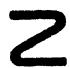
\includegraphics[keepaspectratio]{images/part001_037a61a5.jpg}}

换句话说，同一集合 X 上不同的一致结构可以诱导同一拓扑。* 例如，在 {]}0, +∞{[} 上，加法一致结构与乘法一致结构（它们是不同的：第三章 § 6 习题 17）诱导同一拓扑。*

另一个例子见 § 2 第 2 目注 1。

命题 2 设 X 是一致空间。对 X 的每个对称一致邻域 V 与 X × X 的每个子集 M，VMV 是 M 在积空间 X × X 中的邻域，且 M 在此空间中的闭包由下列公式给出

\[
\overline {{\mathbf {M}}} = \bigcap_ {\mathbf {V} \in \mathfrak {S}} \mathbf {V M V}\tag{I}
\]

其中 \(\mathfrak{S}\) 表示 \(\mathbf{X}\) 的对称一致邻域组成的集。

设 V 是 X 的一个对称一致邻域。关系 \((x, y) \in \text{VMV}\) 表示存在 M 的元素 \((p, q)\) 使 \((x, p) \in V\) 且 \((q, y) \in V\)：换句话说（因 V 对称），\(x \in V(p)\) 且 \(y \in V(q)\)，即 \((x, y) \in V(p) \times V(q)\)。由于 \(V(p) \times X(q)\) 是 \((p, q)\) 在 \(X \times X\) 中的邻域，命题的第一部分得证。关系 \((x, p) \in V\) 与 \((y, q) \in V\) 也可写成 \(p \in V(x)\)、\(q \in V(y)\) 或 \((p, q) \in V(x) \times V(y)\)。当 V 取遍 S 时，诸集合 \(V(x) \times V(y)\) 构成 \((x, y)\) 在 \(X \times X\) 中的基本邻域系；因为若 U 与 \(U'\) 是任意两个一致邻域，总存在对称一致邻域 \(V \subset U \cap U'\)，使 \(V(x) \times V(y) \subset U(x) \times U'(y)\)。因此，\(V(x) \times V(y)\) 对每个 \(V \in S\) 都与 M 相交，当且仅当 \((x, y) \in \overline{\mathbf{M}}\)，由此即得公式 (1)。

推论 1 若 A 是 X 的任一子集，V 是 X 的任一对称一致邻域，则 V(A) 是 A 在 X 中的邻域，且

\[
\overline {{{\mathbf {A}}}} = \bigcap_ {\mathbf {v} \in \mathfrak {S}} \mathbf {V} (\mathbf {A}) = \bigcap_ {\mathbf {v} \in \mathfrak {U}} \mathbf {V} (\mathbf {A})\tag{2}
\]

其中 \(\mathfrak{U}\) 表示 \(\mathbf{X}\) 中所有一致邻域组成的集。

若 \(\mathbf{M} = \mathbf{A} \times \mathbf{A}\)，则 \(\mathrm{VMV} = \mathrm{V}(\mathbf{A}) \times \mathrm{V}(\mathbf{A})\) 对任何 \(\mathbf{V} \in \mathfrak{S}\) 成立；因为关系“存在 \(p \in \mathbf{A}\) 使 \((x, p) \in \mathbf{V}"\)按定义等价于 \(x \in \mathbf{V}(\mathbf{A})\)。推论由第一章 § 4 第 2 目命题 5 与第 3 目命题 7 立即得出。

V(A) 称为 A 的 V-邻域。

若 V 是在 X × X 中开的一致邻域，则对每个 x ∈ X，V(x) 在 X 中开（第一章 § 4 第 2 目命题 4 的推论），因此 V(A)——它是 x 取遍 A 时诸 V(x) 的并——在 X 中开。另一方面，若 V 是 X × X 中的闭一致邻域，则对 X 的每个子集 A，V(A) 未必在 X 中闭（习题 3）。

\pandocbounded{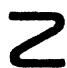
\includegraphics[keepaspectratio]{images/part001_f8cd4ad5.jpg}}

还应指出，当 V 取遍 X 的一致邻域集时，诸集合 V(A) 未必构成 A 在 X 中的基本邻域系（习题 2）。

推论 2 X 的一致邻域在 X × X 中的内部（相应地，闭包）构成 X 的一个一致邻域基本系。

若 V 是 X 的任一一致邻域，则存在对称一致邻域 W 使 \(W \subset V\)；由于 W 是 W 的邻域（命题 2），V 在 \(X \times X\) 中的内部含 W，从而是一个一致邻域。此外，由命题 2 有 \(W \subset W \subset W \subset V\)，因此 V 含某个一致邻域的闭包。

推论 3 每个一致空间都满足公理（O \(_{III}\)）。

若 \(x\) 是 \(X\) 的任一点且 \(V\) 取遍 \(X\) 的在 \(X \times X\) 中闭的一致邻域，则由推论 2，诸集合 \(V(x)\) 构成 \(x\) 在 \(X\) 中的基本邻域系，并且它们在 \(X\) 中闭（第一章 § 4 第 2 目命题 4 的推论）。

命题 3 一致空间 X 是分离的，当且仅当其一致结构的所有一致邻域之交是对角线 \(\Delta\)（即 \(X \times X\) 的对角线）。每个分离的一致空间都是正则的。

后一断言由命题 2 的推论 3 立即得出。我们已看到，闭的一致邻域构成一个一致邻域基本系（命题 2 推论 2）；若其交是 \(\Delta\)，则 \(\Delta\) 在 \(X \times X\) 中闭，从而 \(X\) 是分离的（第一章 § 8 第 1 目命题 1）。反之，若 \(X\) 分离，则对每个点 \((x, y) \notin \Delta\)，存在 \(V\)（\(X\) 的一致邻域）使 \(y \notin V(x)\)，或等价地 \((x, y) \notin V\)；于是 \(\Delta\) 是所有一致邻域之交。

若一致空间 X 分离，我们就说 X 的一致结构是分离的。若 B 是该结构的一个一致邻域基本系，则 X 分离当且仅当 B 中所有集合之交是 \(\Delta\)。

\section{一致连续函数}

\subsection{一致连续函数}

定义 1 设 \(f\) 是一致空间 \(\mathbf{X}\) 到一致空间 \(\mathbf{X}'\) 的映射；如果对每个 \(\mathbf{V}'\)（\(\mathbf{X}'\) 的一致邻域），存在 \(\mathbf{V}\)（\(\mathbf{X}\) 的一致邻域），使关系 \((x,y)\in \mathbf{V}\) 蕴含 \((f(x),f(y))\in \mathbf{V}'\)，则称 f 为一致连续的。

用更形象的说法：\(f\) 一致连续，是指 \(f(x)\) 与 \(f(y)\) 要多接近就有多接近，只要 \(x\) 与 \(y\) 足够接近。

若令 \(g = f \times f\)，则定义 1 的意思是：只要 \(V'\) 是 \(X'\) 的一致邻域，\(\overline{g}^1(V')\) 就是 \(X\) 的一致邻域。

例。1）一致空间到其自身的恒等映射是一致连续的。

\begin{enumerate}
\def\labelenumi{\arabic{enumi})}
\setcounter{enumi}{1}
\item
  一致空间到一致空间的常值映射是一致连续的。
\item
  离散一致空间到一致空间的每个映射都是一致连续的。
\end{enumerate}

命题 1 每个一致连续映射都是连续的。

这是定义的直接推论。

另一方面，一致空间 X 到一致空间 \(X'\) 的连续映射未必一致连续，* 例如 \(x \to x^{3}\)，它是 R 到自身的同胚，但关于加法一致结构不一致连续。*（见 § 4 第 1 目定理 2。）

命题 2 （a）若 \(f: \mathbf{X} \to \mathbf{X}'\) 与 \(g: \mathbf{X}' \to \mathbf{X}''\) 是两个一致连续映射，则 \(g \circ f: \mathbf{X} \to \mathbf{X}''\) 是一致连续的。

\begin{enumerate}
\def\labelenumi{(\alph{enumi})}
\setcounter{enumi}{1}
\tightlist
\item
  设 \(f\) 是一致空间 \(\mathbf{X}\) 到一致空间 \(\mathbf{X}'\) 上的双射；它是同构，当且仅当 \(f\) 与 \(f\) 的逆映射都一致连续。
\end{enumerate}

这由定义 1 借助积映射 \(f \times f\) 的解释立即得出。

\subsection{一致结构的比较}

第 1 目的命题 2 表明，我们可以取一致连续映射作为一致结构的态射（《集合论》，第四章，§ 2，第 1 目）；今后我们总假定态射就是这样选取的。按照一般的定义（《集合论》，第四章，§ 2，第 2 目），这使我们可以对给定集合 X 上的一切一致结构组成的集定义一个序关系：

定义 2 若 \(\mathfrak{U}_1\) 与 \(\mathfrak{U}_2\) 是同一集合 \(\mathbf{X}\) 上的两个一致结构，则称 \(\mathfrak{U}_1\) 比 \(\mathfrak{U}_2\) 细（而 \(\mathfrak{U}_2\) 比 \(\mathfrak{U}_1\) 粗），如果记 \(\mathbf{X}_i\) 为集合 \(\mathbf{X}\) 赋以一致结构 \(\mathfrak{U}_i\) 后所得的空间（ \(i = 1,2\)），恒等映射 \(\mathbf{X}_1 \to \mathbf{X}_2\) 一致连续。

若 \(\mathfrak{U}_1\) 比 \(\mathfrak{U}_2\) 细且异于 \(\mathfrak{U}_2\)，则称 \(\mathfrak{U}_1\) 严格地细于 \(\mathfrak{U}_2\)（而 \(\mathfrak{U}_2\) 严格地粗于 \(\mathfrak{U}_1\)）。

两个一致结构称为可比较的，如果其中一个比另一个细。

例。在集合 X 上一切一致结构组成的有序集中，离散一致结构是最细的，而最粗的一致结构是其一致邻域集由单个元素 \(X \times X\) 组成的那一个。

下述命题是第 1 目定义 1 的直接推论：

命题 3 若 \(\mathfrak{U}_1\) 与 \(\mathfrak{U}_2\) 是集合 \(X\) 上的两个一致结构，则 \(\mathfrak{U}_1\) 比 \(\mathfrak{U}_2\) 细，当且仅当 \(\mathfrak{U}_2\) 的每个一致邻域都是 \(\mathfrak{U}_1\) 的一致邻域。

推论 设 \(\mathfrak{U}_1\) 与 \(\mathfrak{U}_2\) 是集合 \(X\) 上的两个一致结构，且设 \(\mathfrak{U}_1\) 比 \(\mathfrak{U}_2\) 细；则 \(\mathfrak{U}_1\) 诱导的拓扑比 \(\mathfrak{U}_2\) 诱导的拓扑细。

这由拓扑按邻域的比较（第一章 § 2 第 2 目命题 3）立即得出。

注。1）可能发生这样的情形：一致结构 \(\mathcal{U}_1\) 严格地细于一致结构 \(\mathcal{U}_2\)，但二者诱导的拓扑相同。下面的例子表明这一点：

设 \(\mathbf{X}\) 是非空集合。对每个有限分拆 \(\varpi = (\mathrm{A}_i)_{1\leqslant i\leqslant n}\)（\(\mathbf{X}\) 的），令 \(\mathrm{V}_{\overline{\omega}}\) 表示

\[
\bigcup_ {i} \mathrm{A} _ {i} \times \mathrm{A} _ {i}.
\]

于是诸集合 \(V_{\overline{w}}\) 构成某个一致结构 \(\mathcal{U}\)（\(X\) 上的）的一致邻域基本系。因为若 \(\varpi\) 是 \(X\) 的任一有限分拆，我们有 \(\Delta \subset V_{\overline{w}}\) 且 \(V_{\overline{w}} \circ V_{\overline{g}} = \overline{V}_{\overline{w}}^{1} = V_{\overline{w}}\)（§ 1 第 1 目例 2）；又若 \(\varpi' = (B_j)\) 与 \(\varpi'' = (C_k)\) 是 \(X\) 的两个有限分拆，则诸集合 \(B_j \cap C_k\) 中非空者构成一个有限分拆 \(\varpi\)（\(X\) 的），并且 \(V_{\overline{w}} \subset V_{\overline{w}'} \cap V_{\overline{w}''}\)。称 \(\mathcal{U}\) 为 \(X\) 上有限分拆的一致结构。由 \(\mathcal{U}\) 诱导的拓扑是离散拓扑，因为对每个 \(x \in X\)，集合 \(\{x\}\) 与 \(C\{x\}\) 构成 \(X\) 的一个有限分拆。然而，若 \(X\) 无限，则显然 \(\mathcal{U}\) 严格地粗于离散一致结构。2）若 \(f: X \to X'\) 是一致连续映射，则 \(f\) 在把 \(X\) 的一致结构换成较细的一致结构、把 \(X'\) 的一致结构换成较粗的一致结构之后仍一致连续（第 1 目命题 2）。换句话说，\(X\) 的一致结构越细且 \(X'\) 的一致结构越粗，\(X\) 到 \(X'\) 的一致连续映射就越多。

\subsection{初始一致结构}

命题 4 设 X 是一个集合，\((\mathrm{Y}_{t})_{t\in I}\) 是一族一致空间，且对每个 \(t\in I\)，\(f_{t}\) 是 X 到 \(Y_{t}\) 的映射。对每个 \(t\in I\)，令 \(g_{t}\) 表示 \(f_{t}\times f_{t}\)。设 S 为 \(X\times X\) 中形如 \(\overline{g}_{t}(V_{t})\) 的子集组成的集，其中 \(t\in I\) 而 \(V_{t}\) 是 \(Y_{t}\) 的一致邻域；又设 B 为一切有限交

\[
\mathbf {U} \left(\mathrm{V} _ {\iota_ {1}}, \dots , \mathrm{V} _ {\iota_ {n}}\right) = _ {i} ^ {- 1} g _ {i} \left(\mathrm{V} _ {\iota_ {1}}\right) \cap \dots \cap^ {- 1} g _ {\iota_ {n}} \left(\mathrm{V} _ {\iota_ {n}}\right)\tag{1}
\]

组成的集，其中每个成员由 \(\mathfrak{S}\) 中的集合构成。于是 \(\mathfrak{B}\) 是某个一致结构 \(\mathfrak{U}\)（\(\mathbf{X}\) 上的）的一致邻域基本系，该一致结构是 \(\mathbf{X}\) 关于族 \((f_{\mathfrak{i}})\) 的初始一致结构（《集合论》，第四章，§ 2，第 3 目），特别地，\(\mathfrak{U}\) 是 \(\mathbf{X}\) 上使所有映射 \(f_{\mathfrak{i}}\) 都一致连续的最粗一致结构。进而言之，设 \(h\) 是一致空间 \(\mathbf{Z}\) 到 \(\mathbf{X}\) 的映射；则 \(h\) 一致连续（当 \(\mathbf{X}\) 赋有一致结构 \(\mathfrak{U}\) 时），当且仅当每个映射 \(f_{\mathfrak{i}} \circ h\) 都一致连续。

立即可以看出 \(\mathfrak{B}\) 满足公理 \((\mathbf{B}_1)\mathbf{Y}\) 与 \((\mathbf{U}_1')\)。若 \(\mathbf{W}_t = \overline{g}_t^1 (\mathbf{V}_t)\)，则 \(\overline{\mathbf{W}}_t = \overline{g}_t^1 (\overline{\mathbf{V}}_t^1)\) 且 \(\dot{\mathbf{W}}_t = \overline{g}_t^1 (\overline{\mathbf{V}}_t^2)\)；于是 \(\mathfrak{B}\) 也满足公理 \((\mathbf{U}_{\mathrm{II}}^t)\) 与 \((\mathbf{U}_{\mathrm{III}}^t)\)，从而是某个一致结构 \(\mathcal{U}\)（\(\mathbf{X}\) 上的）的一致邻域基本系。此外，由 \(\mathcal{U}\) 的定义以及第 1 目的定义 1 立即可知，\(f_{t}\) 对每个指标 \(i\in I\) 一致连续；因此（第 1 目命题 2）\(f_{t}\circ h\) 对每个 \(i\in I\) 都一致连续，只要 \(h\) 一致连续。反之，设 \(f_{t}\circ h\) 对每个 \(i\in I\) 都一致连续，并考虑一个集合 \(\mathrm{U}(\mathrm{V}_{i_t},\dots,\mathrm{V}_{i_n})\)；由假设，对每个 \(k\)（\(1\leqslant k\leqslant n\)），存在 \(\mathbf{W}_k\)（\(\mathbf{Z}\) 的一致邻域），使关系 \((z,z^{\prime})\in \mathbf{W}_k\) 蕴含 \([f_{i_k}(h(z)),f_{i_k}(h(z')))]\in \mathbf{V}_k\)；若

\[
\mathbf {W} = \bigcap_ {k} \mathbf {W} _ {k},
\]

则这 \(n\) 个关系只要 \(z\) 与 \(z'\) 是 W-邻近的便同时满足，从而有 \((h(z), h(z')) \in \mathrm{U}(\mathrm{V}_{\iota_1}, \ldots, \mathrm{V}_{\iota_n})\)，证明完成。

推论 使诸 \(f_{i}\) 一致连续的最粗一致结构 U 在 X 上诱导的拓扑，也是使诸 \(f_{i}\) 连续的最粗拓扑。

这是后一拓扑中一点的邻域定义（第一章 § 2 第 3 目命题 4）的直接推论。

初始结构的一般性质（《集合论》，第四章，§ 2，第 3 目，判别准则 CST 10）特别蕴含下列传递性质：

命题 5 设 X 是一个集合，\((Z_{\iota})_{\iota \in I}\) 是一族一致空间，\((J_{\lambda})_{\lambda \in L}\) 是 I 的一个分拆，\((Y_{\lambda})_{\lambda \in L}\) 是以 L 为指标集的一族集合。对每个 \(\lambda \in L\)，设 \(h_{\lambda}\) 是 X 到 \(Y_{\lambda}\) 的映射；对每个 \(\lambda \in L\) 与每个 \(\iota \in J_{\lambda}\)，设 \(g_{\iota \lambda}\) 是 \(Y_{\lambda}\) 到 \(Z_{\iota}\) 的映射；并令 \(f_{\iota} = g_{\iota \lambda} \circ h_{\lambda}\)。设每个 \(Y_{\lambda}\) 赋有使诸映射 \(g_{\iota \lambda} (\iota \in J_{\lambda})\) 一致连续的最粗一致结构。则使诸 \(f_{\iota}\) 一致连续的 X 上最粗的一致结构，与使诸 \(h_{\lambda}\) 一致连续的 X 上最粗的一致结构是同一个。

\subsection{一致结构的逆像；一致子空间}

设 X 是一个集合，Y 是一致空间，f 是 X 到 Y 的映射。X 上使 f 一致连续的最粗一致结构 U 称为 Y 的一致结构在 f 下的逆像。由第 3 目的命题 4 以及给出交的逆像的公式可知，Y 的一致邻域在 \(g = f \times f\) 下的诸逆像构成 U 的一致邻域基本系。由 U 诱导的拓扑是 Y 的拓扑在 f 下的逆像（第 3 目命题 4 的推论）。

注 若 \(f: \mathbf{X} \to \mathbf{Y}\) 是满射，则 \(\mathbf{Y}\) 的一致邻域是在 \(g\) 之下 \(\mathbf{X}\) 的一致邻域的直接像。

设 \(f\) 是一致空间 \(\mathbf{X}\) 到一致空间 \(\mathbf{X}'\) 的映射；它一致连续的充要条件是：在 \(f\) 之下 \(\mathbf{X}'\) 的一致结构的逆像粗于 \(\mathbf{X}\) 的一致结构。

设 A 是一致空间 X 的子集。X 的一致结构在 A 上诱导的一致结构是后者在典范单射 \(A \rightarrow X\) 下的逆像。由第 3 目命题 4，这等价于下述定义：

定义 3 设 A 是一致空间 X 的子集。A 上以 X 的一致邻域集在 A × A 上的迹为一致邻域集的那个一致结构，称为 X 的一致结构在 A 上诱导的一致结构。

由 A 上诱导的一致结构所诱导的拓扑，与 X 的拓扑在 A 上诱导的拓扑相同；集合 A 连同由 X 的一致结构与拓扑诱导的一致结构与拓扑，称为 X 的一致子空间。

若 A 是一致空间 X 的子集，且 \(f: X \to X'\) 是一致连续映射，则限制 \(f|A\) 是 A 到 \(X'\) 的一致连续映射。若 \(A' \subset X'\) 使得 \(f(X) \subset A'\)，则 X 到一致子空间 \(A'\)（\(X'\) 的）中的、与 f 有同一图像的那个映射仍一致连续（第 3 目命题 4）。

若 \(B \subset A \subset X\)，则 X 的一致子空间 B 与 X 的一致子空间 A 的一致子空间 B 相同（诱导一致结构的可递性；第 3 目命题 5）。

命题 6 设 A 是一致空间 X 的稠密子集。则一致子空间 A 的诸一致邻域在 X × X 中的闭包构成 X 的一致邻域基本系。

A × A 在 X × X 中稠密（第一章 § 4 第 3 目命题 7）。设 V 是 A 的一个开一致邻域；它是 A × A 与 X 的某个开一致邻域 U 的交。我们有 U ⊂ V̄（第一章 § 1 第 6 目命题 5），而这一关系与 V̄ ⊂ U 合在一起，依据 § 1 第 2 目命题 2 的推论 2，便证明了本命题。

\subsection{一致结构集的上确界}

每个族 \((\mathcal{U}_t)_{i\in I}\)（集合 \(X\) 上的一致结构族）都有上确界 \(\mathcal{U}\)，这里所指的有序集是 \(X\) 上所有一致结构组成的有序集；只需应用第 3 目命题 4，取 \(Y_t\) 为集合 \(X\) 赋以一致结构 \(\mathcal{U}_t\) 后所得的空间，并取 \(f_t\) 为恒等映射 \(X\to Y_t\)。由 \(\mathcal{U}\) 诱导的拓扑恰是由诸 \(\mathcal{U}_t\) 诱导的拓扑的上确界。

由第 3 目命题 4 还可得出：若 X 非空且 \(\mathcal{U}_{t}\) 是 \(\mathcal{U}_{t}\) 的一致邻域滤子，则 \(\mathcal{U}\) 的一致邻域滤子是诸滤子 \(\mathcal{U}_{t}\) 的上确界（第一章 § 6 第 2 目）。

例 若 \(\varpi\) 是任一有限分拆 \((\mathbf{A}_i)_{1 \leqslant i \leqslant n}\)（非空集合 \(\mathbf{X}\) 的），则集合 \(\mathbf{V}_{\overline{\omega}} = \bigcup_{i} (\mathbf{A}_i \times \mathbf{A}_i)\) 本身就构成

X 上某个一致结构 \(\mathfrak{U}_{\varpi}\) 的一致邻域基本系（§ 1 第 1 目例 2）；X 上有限分拆的一致结构（第 2 目注 1）就是诸一致结构 \(\mathfrak{U}_{\varpi}\) 的上确界。

注 X 上的一致结构族 \((\mathcal{U}_{i})\) 在 X 上所有一致结构组成的有序集中也有下确界，即由 X 上粗于每个 \(U_{i}\) 的一切一致结构组成的集的上确界（这样的一致结构存在，因为 X 上所有一致结构组成的集有最小元素）。但是（设 X 非空）这一一致结构的一致邻域滤子未必是诸 \(U_{i}\) 的一致邻域滤子的交，因为后一滤子未必满足公理 \((\mathrm{U}_{\mathrm{III}})\)（习题 4）。

\subsection{一致空间的积}

定义 4 若 \((\mathbf{X}_t)_{i\in I}\) 是一族一致空间，则该族的积一致空间是指积集合

\[
\mathbf {X} = \prod_ {i \in I} \mathbf {X} _ {i}
\]

并赋以使诸投影 \(pr_{t}: X \rightarrow X_{t}\) 都一致连续的最粗一致结构。这一一致结构称为诸 \(X_{t}\) 的一致结构的积，而一致空间 \(X_{t}\) 称为 X 的因子。

积一致结构在 X 上诱导的拓扑与诸 \(X_{i}\) 的拓扑的积相同（第 3 目命题 4 的推论）。

命题 7 设 \(f = (f_{t})\) 是一致空间 \(Y\) 到积一致空间 \(X = \prod_{i \in I} X_{i}\) 的映射。则 \(f\) 一致连续当且仅当每个 \(f_{t}\) 都一致连续。

由于 \(f_{i} = \mathrm{pr}_{i} \circ f\)，这是第 3 目命题 4 的一个特殊情形。

推论 设 \((\mathbf{X}_t)_{i \in I}, (\mathbf{Y}_t)_{i \in I}\) 是以同一集 I 为指标的两族一致空间。对每个 \(i \in I\)，设 \(f_t\) 是 \(\mathbf{X}_t\) 到 \(\mathbf{Y}_t\) 的映射。若每个 \(f_t\) 都一致连续，则积映射

\[
f: (x _ {i}) \rightarrow (f _ {i} (x _ {i})).
\]

反之，若诸 \(X_{i}\) 非空且 f 一致连续，则每个 \(f_{i}\) 都一致连续。

\(f\) 可写成 \(x \to (f_{i}(\mathrm{pr}_{i}x))\)，因此推论的第一部分由命题 7 得出。第二部分的证明：考虑一点 \(a = (a_{i})\)（属于 \(\prod_{i \in I} X_{i}\)），并重复第一章 § 4 第 1 目命题 1 推论 1 的论证，把其中“在 \(a\)（相应地，\(a_{x}\)）连续”一语换成“一致连续”。

初始一致结构的可递性的一般判据（第 3 目命题 5）表明，如同拓扑空间的积的情形一样（第一章 § 4 第 1 目），一致空间的积是可结合的，并且下述结论成立：

命题 8 设 X 是一个集合，\((\mathbf{Y}_t)_{t \in I}\) 是一族一致空间，且对每个 \(t \in I\)，\(f_t\) 是 X 到 \(\mathbf{Y}_t\) 的映射。设 \(f\) 是映射 \(x \to (f_t(x))\)（从 X 到 \(\mathbf{Y} = \prod_{t \in I} \mathbf{Y}_t\)），并设 \(\mathfrak{U}\) 是 X 上使诸 \(f_t\) 一致连续的最粗一致结构。则 \(\mathfrak{U}\) 是在 \(f\) 之下，Y 的积一致结构在 \(f(\mathbf{X})\) 上诱导的一致结构的逆像。

推论 对每个 \(i \in I\)，设 \(A_{i}\) 是 \(Y_{i}\) 的子空间。则在 \(A = \prod_{i \in I} A_{i}\) 上由 \(\prod_{i \in I} Y_{i}\) 的积一致结构所诱导的一致结构，与诸子空间 \(A_{i}\) 的一致结构的积相同。

此外，立即可以看出，若 \(X_{1}, X_{2}\) 是两个一致空间而 \(a_{1}\) 是 \(X_{1}\) 的任意一点，则映射 \(x_{2} \to (a_{1}, x_{2})\) 是 \(X_{2}\) 到子空间 \(\{a_{1}\} \times X_{2}\)（\(X_{1} \times X_{2}\) 的）上的同构；因此：

命题 9 设 \(f\) 是积一致空间 \(\mathbf{X}_1 \times \mathbf{X}_2\) 到一致空间 \(\mathbf{Y}\) 的一致连续映射；则每个偏映射

\[
x _ {2} \rightarrow f (x _ {1}, x _ {2})
\]

（作为 \(X_{2}\) 到 Y 的映射）都是一致连续的。

换言之，两个变元的一致连续函数对每个变元分别是一致连续的。

* 第一章 § 4 第 2 目注 2 中给出的例子表明，本命题的逆命题不成立。 *

\subsection{一致空间的逆极限}

设 I 是一个偏序集，其偏序记作 \(\alpha \leqslant \beta\)。对每个 \(\alpha \in I\)，设 \(X_{\alpha}\) 是一致空间；又对每对指标 \(\alpha, \beta\)（满足 \(\alpha \leqslant \beta\)），设 \(f_{\alpha \beta}\) 是 \(X_{\beta}\) 到 \(X_{\alpha}\) 的映射。

我们称 \((\mathbf{X}_{\alpha}, f_{\alpha\beta})\) 是一致空间的逆系统，如果 (i) \((\mathbf{X}_{\alpha}, f_{\alpha\beta})\) 是集合的逆系统（参见第一章附录第 1 目），且 (ii) 只要 \(\alpha \leqslant \beta\)，\(f_{\alpha\beta}\) 就是一致连续的。在 \(X = \varprojlim X_{\alpha}\) 上，使诸典范映射 \(f_{\alpha}: X \to X_{\alpha}\) 都一致连续的最粗一致结构，称为（关于 \(f_{\alpha\beta}\) 的）诸 \(X_{\alpha}\) 的一致结构的逆极限；赋有这一最粗一致结构的集合 X 称为一致空间的逆系统 \((\mathbf{X}_{\alpha}, f_{\alpha\beta})\) 的逆极限。第一章 § 4 第 4 目中建立的拓扑空间逆极限的所有性质（命题 9 除外）在把“拓扑”换成“一致结构”、“连续映射”换成“一致连续映射”之后仍然成立。此外：

命题 10 设 I 是有向集，\((\mathbf{X}_{\alpha}, f_{\alpha \beta})\) 是以 I 为指标的一致空间逆系统，J 是 I 的共尾子集。对每个 \(\alpha \in I\)，设 \(f_{\alpha}\) 是 \(\mathbf{X} = \varprojlim \mathbf{X}_{\alpha}\) 到 \(\mathbf{X}_{\alpha}\) 的典范映射，并用 \(g_{\alpha}\) 表示 \(f_{\alpha} \times f_{\alpha}\)。则集合族 \(\overline{g}_{\alpha}^{1}(\mathrm{V}_{\alpha})\)（其中 \(\alpha\) 取遍 J，且对每个 \(\alpha \in J\)，\(\mathrm{V}_{\alpha}\) 取遍 \(\mathrm{X}_{\alpha}\) 的一个一致邻域基本系）构成 X 的一致邻域基本系。

证明留给读者；它只需把第一章 § 4 第 4 目命题 9 的证明直接加以改编。

最后，在 \(X = \varprojlim X_{\alpha}\) 上由诸 \(X_{\alpha}\) 的一致结构的逆极限所诱导的拓扑，就是诸 \(X_{\alpha}\) 的拓扑的逆极限。

\section{完备空间}

\subsection{Cauchy 滤子}

一旦集合 X 赋有了一致结构，我们就可以定义（相对于该结构的）X 的“小”子集指的是什么：X 的“小”子集是指其中所有点彼此“非常接近”的那种子集。精确地说：

定义 1 若 X 是一致空间而 V 是 X 的一致邻域，则称 X 的子集 A 是 V-小集，如果 A 的任意两点都 V-邻近（换言之，A × A ⊂ V）。

命题 1 在一致空间 X 中，若两个集合 A 与 B 都是 V-小集且相交，则其并 A ∪ B 是 V-小集。

设 \(x\) 与 \(y\) 是 \(A \cup B\) 的任意两点，并设 \(Z \in A \cap B\)。则 \((x, z) \in V\) 且 \((z, y) \in V\)，从而 \((x, y) \in \mathring{V}\)。

定义 2 滤子 \(\mathfrak{F}\)（一致空间 \(\mathbf{X}\) 上的）称为 Cauchy 滤子，如果对 X 的每个一致邻域 V，存在 X 的一个子集，它是 V-小集且属于 \(\mathfrak{F}\)。

这里我们同样可以借助“足够小的集合”与“要多小有多小的集合”这些说法使语言更形象；于是定义 2 可以改述为：Cauchy 滤子就是包含任意小的集合的滤子。

无穷序列 \((u_n)\)（一致空间 \(X\) 的点列）称为 Cauchy 序列，如果与该序列相伴的初等滤子是 Cauchy 滤子。这等价于说：对每个一致邻域 \(V\)（\(X\) 的），存在整数 \(n_0\)，使得对一切满足 \(m \geqslant n_0\) 与 \(n \geqslant n_0\) 的整数 m 与 n，都有 \((u_m, u_n) \in V\)。

命题 2 在一致空间 X 上，每个收敛滤子都是 Cauchy 滤子。

若 \(x\) 是 \(X\) 的任意一点，且 \(V\) 是 \(X\) 的任意对称一致邻域，则邻域 \(V(x)\)（\(x\) 的）是 \(V\)-小集。若 \(\mathfrak{F}\) 是收敛于 \(x\) 的滤子，则 \(\mathfrak{F}\) 中有一个集合含于 \(V(x)\)，因而是 \(V\)-小集。

显然，每个细于某个 Cauchy 滤子的滤子都是 Cauchy 滤子。

命题 3 设 \(f: \mathbf{X} \to \mathbf{X}'\) 是一致连续映射。则在 \(f\) 之下，\(\mathbf{X}\) 上 Cauchy 滤子基的像是 \(\mathbf{X}'\) 上的 Cauchy 滤子基。

设 \(g = f \times f\)。若 \(V'\) 是 \(X'\) 的一致邻域，则 \(\overline{g}^1(V')\) 是 \(X\) 的一致邻域，且在 \(f\) 之下，\(\overline{g}^1(V')\)-小集的像是 \(V'\)-小集；由此即得结论。

特别由此可得：若把一致空间 X 的一致结构换成较粗的一致结构，则关于原来一致结构的每个 Cauchy 滤子关于新一致结构仍是 Cauchy 滤子。

这一事实很容易按下述形式记住：一致结构越细，Cauchy 滤子就越少。

命题 4 设 X 是一个集合，\((\mathbf{Y}_i)_{i\in I}\) 是一族一致空间，且对每个 \(i\in I\)，\(f_i\) 是 X 到 \(\mathbf{Y}_i\) 的映射。设 X 赋有最粗的一致结构 \(\mathcal{U}\)，使诸 \(f_i\) 都一致连续。则 X 上的滤子基 \(\mathcal{B}\) 是 Cauchy 滤子基的充要条件是：\(f_i(\mathcal{B})\) 是 \(\mathbf{Y}_i\) 上的 Cauchy 滤子基（对每个 \(i\in I\)）。

由命题 3，条件是必要的。反之，设条件满足，并设 \(\mathbf{U}(\mathbf{V}_{\iota_1},\ldots ,\mathbf{V}_{\iota_n})\) 是一致结构 \(\mathfrak{U}\) 的一个一致邻域{[}§ 2 第 3 目公式 (1){]}。由假设，对每个指标 \(k\)，存在集合 \(\mathbf{M}_k\in \mathfrak{B}\)，使 \(f_{\iota_k}(\mathbf{M}_k)\) 是 \(\mathbf{V}_{\iota_k}\)-小集 ( \(\iota \leqslant k\leqslant n\) )。设 \(\mathbf{M}\) 是 \(\mathfrak{B}\) 中含于诸 \(\mathbf{M}_k\)（\(\iota \leqslant k\leqslant n\)）的一个集合；则对每对点 \(x,x^{\prime}\)（\(\mathbf{M}\) 的），有 \([f_{\iota_k}(x),f_{\iota_k}(x')]\in \mathbf{V}_{\iota_k}\)（\(\iota \leqslant k\leqslant n\)），从而

\[
(x, x ^ {\prime}) \in \mathrm{U} (\mathrm{V} _ {t _ {1}}, \dots , \mathrm{V} _ {t _ {n}}).
\]

证明完毕。

推论 1 若一致空间 X 上的 Cauchy 滤子在 X 的子集 A 上诱导出一个滤子，则该滤子是一致子空间 A 上的 Cauchy 滤子。

推论 2 滤子基 \(\mathfrak{B}\)（一致空间的积 \(\prod_{i\in I}X_i\) 上的）是 Cauchy 滤子基的充要条件是：对每个 \(i\in I\)，\(\operatorname{pr}_i(\mathfrak{B})\) 是 \(X_i\) 上的 Cauchy 滤子基。

\subsection{极小 Cauchy 滤子}

一致空间 X 上 Cauchy 滤子组成的集的（关于包含关系的）极小元素，称为 X 上的极小 Cauchy 滤子。

命题 5 设 X 是一致空间。对 X 上每个 Cauchy 滤子 F，存在唯一的粗于 F 的极小 Cauchy 滤子 \(\mathfrak{F}_0\)。若 B 是 F 的基，S 是 X 的对称一致邻域的一个基本系，则诸集合 V(M)（M ∈ B, V ∈ S）构成 \(\mathfrak{F}_0\) 的一个基。

若 M 与 \(M'\) 属于 B，V 与 \(V'\) 属于 S，则存在集合 \(M'' \in B\)（相应地 \(V'' \in S\)），使 \(M'' \subset M \cap M'\)（相应地 \(V'' \subset V \cap V'\)）；于是 \(V''(M'') \subset V(M) \cap V'(M')\)，因而诸集合 \(V(M)\)（ \(M \in B\)，\(V \in S\) ）确实构成 X 上一个滤子 \(F_0\) 的基。进而，若 M 是 V-小集，

则 V(M) 是 V-小集；因此 \(\mathfrak{F}_0\) 是 Cauchy 滤子，且显然粗于 \(\mathfrak{F}\)。为完成证明，只需证明：若 \(\mathfrak{G}\) 是粗于 \(\mathfrak{F}\) 的 Cauchy 滤子，则 \(\mathfrak{G}\) 细于 \(\mathfrak{F}_0\)。对每个 M ∈ \(\mathfrak{B}\) 与每个 V ∈ \(\mathfrak{S}\)，存在一个 V-小集 N ∈ \(\mathfrak{G}\)；由于 N ∈ \(\mathfrak{F}\)，N 与 M 相交；于是 N ⊂ V(M)，从而 V(M) ∈ \(\mathfrak{G}\)。

推论 1 对每个 \(x \in \mathbf{X}\)，邻域滤子 \(\mathfrak{B}(x)\)（\(x\) 在 \(\mathbf{X}\) 中的）是极小 Cauchy 滤子。

在命题 5 中取 \(\mathfrak{F}\) 为 \(\mathbf{X}\) 中含 \(x\) 的一切子集组成的滤子，并取 \(\mathfrak{B}\) 由单个元素 \(\{x\}\) 组成。

推论 2 Cauchy 滤子 F 的每个聚点 x 都是 F 的极限点。

存在一个滤子 \(\mathfrak{G}\)，它既细于 \(\mathfrak{F}\) 又细于 \(\mathfrak{B}(x)\)（第一章 § 7 第 2 目命题 4）；由于 \(\mathfrak{F}\) 是 Cauchy 滤子，\(\mathfrak{G}\) 也是。若 \(\mathfrak{F}_0\) 是粗于 \(\mathfrak{F}\) 的唯一的极小 Cauchy 滤子，则 \(\mathfrak{F}_0\) 与 \(\mathfrak{B}(x)\) 都是粗于 \(\mathfrak{G}\) 的极小 Cauchy 滤子。因此 \(\mathfrak{F}_0 = \mathfrak{B}(x)\)，这表明 \(\mathfrak{F}\) 收敛于 \(x\)。

推论 3 凡粗于某个收敛于点 x 的滤子的 Cauchy 滤子，也收敛于 x。

这是推论 2 的一个推论。

推论 4 若 \(\mathfrak{F}\) 是极小 Cauchy 滤子，则 \(\mathfrak{F}\) 的每个集合都有非空的内部，且该内部也属于 \(\mathfrak{F}\)（换言之，\(\mathfrak{F}\) 具有一个由开集组成的基）。

设 V 是 X 的任一一致邻域；则存在开的一致邻域 \(U \subset V\)（§ 1 第 2 目命题 2 的推论 2）。对 X 的每个子集 M，\(U(M)\) 是开集且含于 \(V(M)\)；于是由命题 5 即得结论。

\subsection{完备空间}

在一致空间 X 中，Cauchy 滤子未必有极限点。

例。1）考虑序列 \((u_{n})\)（在有理直线 \(\mathbf{Q}\) 上），它由下式定义：

\[
\text { by } \quad u _ {n} = \sum_ {p = 0} 2 ^ {- p (p + 1) / 2}. \quad \text { If } \quad m > n \quad \text { we   have }\tag{1}
\]

\[
\left| u _ {m} - u _ {n} \right| \leqslant 2 ^ {- n (n + 3) / 2}
\]

因而 \((u_{n})\) 是 Cauchy 序列。但这一序列在 \(\mathbf{Q}\) 中没有极限；因为若有理数 \(a / b\) 是 \((u_{n})\) 的极限，则由 (1)，对所有 \(n\) 我们应有

\[
\left| a / b - h _ {n} / 2 ^ {n (n + 1) / 2} \right| \leqslant 1 / 2 ^ {n (n + 3) / 2}
\]

其中 \(h_n\) 是（依赖于 \(n\) 的）整数；即

\[
\left| a. 2 ^ {n (n + 1) / 2} - b h _ {n} \right| \leqslant b. 2 ^ {- n}
\]

对所有 n 成立。现在，对一切 n，这一不等式的左端都是整数，因而只要 n 大于某个整数 \(n_{0}\)（满足 \(b < 2^{n_{0}}\)），它就必须为零；于是应有 \(a/b = u_{n}\)（对所有 \(n > n_{0}\)），这是荒谬的。

\begin{enumerate}
\def\labelenumi{\arabic{enumi})}
\setcounter{enumi}{1}
\tightlist
\item
  设 X 是无穷集合，并考虑 X 上有限分拆的一致结构（§ 2 第 2 目注 1）。X 上的每个超滤子 F 都是
\end{enumerate}

关于这一一致结构的 Cauchy 滤子。因为若 \((\mathbf{A}_{i})\) 是 X 的一个有限分拆，且

\[
\mathbf {V} = \bigcup_ {i} (\mathbf {A} _ {i} \times \mathbf {A} _ {i})
\]

是其对应的一致邻域，则至少有一个 \(A_{i}\) 属于 F（第一章 § 6 第 4 目命题 5 的推论），而 \(A_{i}\) 是 V-小集。另一方面，X 是无穷离散空间，因而不是紧的，从而 X 上存在不收敛的超滤子。

定义 3 完备空间是指每个 Cauchy 滤子都收敛的一致空间。

因此，在完备空间中，每个 Cauchy 序列（第 1 目）都收敛。例 在离散一致空间 X 上，Cauchy 滤子是平凡超滤子（第一章 § 6 第 4 目），因而收敛；从而 X 是完备的。

由第 1 目的定义 2 与定义 3 以及第 1 目的命题 2，我们推出下述命题，它称为 Cauchy 判别准则：

命题 6 设 \(\mathfrak{F}\) 是集合 X 上的滤子，\(f\) 是 X 到完备一致空间 \(\mathbf{X}'\) 的映射。则 \(f\) 关于 \(\mathfrak{F}\) 有极限的充要条件是：\(\mathfrak{F}\) 在 \(f\) 下的像是 Cauchy 滤子基。

这一判别准则表明了完备空间在涉及极限概念的一切问题中的重要性：如果一个函数在完备空间中取值，我们就可以在事先不知道极限值的情况下证明极限的存在；倘若极限的定义是我们掌握的仅有的收敛判别准则，这就不可能做到。

细于完备空间的一致结构的一致结构，未必是完备空间的一致结构（习题 2）。然而，我们有下述命题：

命题 7 设 \(\mathcal{U}_1, \mathcal{U}_2\) 是集合 \(X\) 上的两个一致结构，\(\mathfrak{C}_1, \mathfrak{C}_2\) 分别是这些一致结构诱导的拓扑。假设 \(\mathcal{U}_1\) 细于 \(\mathcal{U}_2\)，且存在 \(\mathcal{U}_1\) 的一个一致邻域基本系，其中的元素作为 \(X \times X\) 的子集在拓扑 \(\mathfrak{C}_2 \times \mathfrak{C}_2\) 中是闭的。则滤子 \(\mathfrak{F}\)（\(X\) 上的）在拓扑 \(\mathfrak{C}_1\) 中收敛的充要条件是：它在一致结构 \(\mathcal{U}_1\) 中是 Cauchy 滤子，且在拓扑 \(\mathfrak{C}_2\) 中收敛。

这些条件显然是必要的，因为 \(\mathfrak{G}_2\) 粗于 \(\mathfrak{G}_1\)。反之，设条件满足，并设 \(x\) 是 \(\mathfrak{F}\) 关于 \(\mathfrak{G}_2\) 的极限点；我们将证明 \(x\) 是 \(\mathfrak{F}\) 关于 \(\mathfrak{G}_1\) 的极限。设 \(V\) 是 \(\mathfrak{U}_1\) 的一个对称一致邻域，它在拓扑 \(\mathfrak{G}_2 \times \mathfrak{G}_2\) 中是闭的。由假设，\(\mathfrak{F}\) 含有一个集合 \(M\)，它是 \(V\)-小集；于是若 \(x' \in M\)，我们就有 \(M \subset V(x')\)。但 \(V(x')\) 在拓扑 \(\mathfrak{G}_{2}\) 中是闭的；因此，\(x\) 位于 \(\mathbf{M}\) 关于 \(\mathfrak{G}_{2}\) 的闭包中，故必属于 \(\mathbf{V}(x')\)。由此得出 \(\mathbf{M} \subset \mathbf{V}(x)\)，命题得证。

推论 在命题 7 的条件下，若 \(\mathfrak{U}_2\) 是完备空间的一致结构，则 \(\mathfrak{U}_1\) 也是完备空间的一致结构。

因为此时每个关于 \(U_{1}\) 的 Cauchy 滤子都是关于 \(U_{2}\) 的 Cauchy 滤子，从而在拓扑 \(G_{2}\) 中收敛。

注意，当 \(\mathcal{C}_1 = \mathcal{C}_2\) 时（§ 1 第 2 目命题 2 的推论 2），命题 7 的推论的假设成立。

\subsection{完备空间的子空间}

命题 8 完备空间的每个闭子空间都是完备的。豪斯多夫一致空间（完备与否）的每个完备子空间都是闭的。

设 X 是完备空间，A 是 X 的闭子空间。若 F 是 A 上的 Cauchy 滤子，则它是 X 上的 Cauchy 滤子基（第 1 目命题 3），因而收敛于某点 \(x \in X\)；但由于 A 是闭的，我们有 \(x \in A\)，因此 F 在子空间 A 中收敛。

现在设 A 是豪斯多夫一致空间 X 的非闭子集，且 \(b \in \overline{\mathbf{A}} - \mathbf{A}\)。b 在 X 中的邻域滤子 B 在 A 上的迹 \(\mathfrak{B}_{\mathbf{A}}\) 是 A 上的 Cauchy 滤子；但它不能收敛于某点 \(c \in \mathbf{A}\)，否则 c 将是 B 的极限点（第 2 目命题 5 推论 3），而这是荒谬的，因为 \(b \neq c\) 且 X 是豪斯多夫的。

命题 9 设 X 是一致空间，A 是 X 的稠密子集，且 A 上每个 Cauchy 滤子基都在 X 中收敛。则 X 是完备的。

只需证明 X 上每个极小 Cauchy 滤子 \(\mathfrak{F}\) 都收敛。由于 A 稠密，且 \(\mathfrak{F}\) 的每个集合都有非空内部（第 2 目命题 5 推论 4），迹 \(\mathfrak{F}_{\mathrm{A}}\)（\(\mathfrak{F}\) 在 A 上的）是 A 上的 Cauchy 滤子，因而收敛于某点 \(x_{0} \in \mathrm{X}\)。由于 \(\mathfrak{F}\) 粗于由 \(\mathfrak{F}_{\mathrm{A}}\) 在 X 上生成的滤子，故 \(\mathfrak{F}\) 收敛于 \(x_{0}\)（第 2 目命题 5 推论 3）。

\subsection{完备空间的积与逆极限}

命题 10 完备一致空间的每个积都是完备的。反之，若非空一致空间的一个积是完备的，则每个因子都是完备一致空间。

第一个断言是积空间上 Cauchy 滤子与收敛滤子的刻画（第 1 目命题 4 推论 2，以及第一章 § 7 第 6 目命题 10 推论 1）的推论。反之，设

\[
\mathbf {X} = \prod_ {i \in I} \mathbf {X} _ {i}
\]

是完备的（诸 \(X_{t}\) 非空），并设 \(F_{x}\) 是 \(X_{x}\) 上的一个 Cauchy 滤子。对每个 \(t \neq x\)，设 \(F_{t}\) 是 \(X_{t}\) 上的一个 Cauchy 滤子，并考虑积滤子（第一章 § 6 第 7 目）

\[
\mathfrak {F} = \prod_ {i \in I} \mathfrak {F} _ {i} \text { on } X;
\]

\(\mathfrak{F}\) 是 Cauchy 滤子（第 1 目命题 4 推论 2），因而是收敛的，从而每个 \(\mathrm{pr}_{\mathbf{x}}\mathfrak{F} = \mathfrak{F}_{\mathbf{x}}\) 也收敛（第一章 § 7 第 6 目命题 10 推论 1）。

推论 设 \((\mathbf{X}_{\alpha}, f_{\alpha\beta})\) 是一致空间的逆系统。若诸 \(X_{\alpha}\) 是豪斯多夫的且完备的，则 \(X = \varprojlim X_{\alpha}\) 也是。

因为 X 是豪斯多夫的，并且可以与 \(\prod_{i\in I}X_{\alpha}\) 的一个闭子空间恒同

（第一章 § 8 第 2 目命题 7 推论 2）；于是该推论由命题 10 与命题 8（第 4 目）得出。

完备豪斯多夫一致空间 \(X_{\alpha}\) 的逆极限可以是空的，即使所有 \(X_{\alpha}\) 都非空且所有 \(f_{\alpha\beta}\) 都是满射，离散空间的情形即表明这一点（《集合论》，第三章，§ 1，习题 32）。然而，我们有下述定理：

定理 1（Mittag-Leffler） 设 \((\mathbf{X}_{\alpha}, f_{\alpha\beta})\) 是完备豪斯多夫一致空间的逆系统，其指标集 I 是具有可数共尾子集的有向集；再设对每个 \(\alpha \in I\)，\(X_{\alpha}\) 具有可数的一致邻域基本系 (*)。最后，设对每个 \(\alpha \in I\)，存在满足下述条件的指标 \(\beta \geqslant \alpha\)：

\((\mathbf{ML}_{\alpha \beta})\) 对每个 \(\gamma \geqslant \beta, f_{\alpha \gamma}(\mathbf{X}_{\gamma})\) 在 \(f_{\alpha \beta}(\mathbf{X}_{\beta})\) 中稠密。

设 \(\mathbf{X} = \varprojlim \mathbf{X}_{\alpha}\)，并设 \(f_{\alpha}\) 是典范映射 \(\mathbf{X} \to \mathbf{X}_{\alpha}\)。则对每个 \(\alpha \in \overleftarrow{\mathbf{I}}\) 与每个 \(\beta \geqslant \alpha\)（满足 \((\mathbf{ML}_{\alpha\beta})\)），\(f_{\alpha}(\mathbf{X})\) 在 \(f_{\alpha\beta}(\mathbf{X}_{\beta})\) 中稠密（因而 \(\mathbf{X}\) 非空，只要诸 \(\mathbf{X}_{\alpha}\) 均非空）。

设 \((\lambda_{n})\) 是 I 中共尾的指标序列。从指标 \(\alpha_0 \in \mathbf{I}\) 出发，递归地定义递增序列 \((\alpha_{n})\)，使 \(\alpha_{n} \geqslant \lambda_{n}\) 且 \((\mathrm{ML}_{\alpha_{n}, \alpha_{n+1}})\) 为真。显然序列 \((\alpha_{n})\) 在 I 中共尾。我们将用 \(f_{mn}\) 代替 \(f_{\alpha_m\alpha_n}\)（当 \(m \leqslant n\) 时），并令 \(f_{n,n+1}(\mathbf{X}_{\alpha_{n+1}}) = \mathbf{Y}_n\)。于是，若 \(m \leqslant n\)，则 \(f_{mn}(\mathbf{Y}_n)\) 在 \(\mathbf{Y}_m\) 中稠密；因为按定义，\(f_{m,n+1}(\mathbf{X}_{\alpha_{n+1}})\) 在

\[
f _ {m, m + 1} \left(\mathrm{X} _ {\alpha_ {m + 1}}\right) = \mathrm{Y} _ {m}, \quad \text { and } \quad f _ {m, n + 1} \left(\mathrm{X} _ {\alpha_ {n + 1}}\right) = f _ {m n} \left[ f _ {n, n + 1} \left(\mathrm{X} _ {\alpha_ {n + 1}}\right) \right] = f _ {m n} \left(\mathrm{Y} _ {n}\right).
\]

对 \(n\) 与 \(k\) 用归纳法，可以定义闭对称一致邻域的基本系 \((\mathbf{V}_{kn})_{k\in \mathbb{N}}\)（\(\mathbf{X}_{\alpha_n}\) 的，对每个 \(n\)），使得

\begin{enumerate}
\def\labelenumi{(\arabic{enumi})}
\setcounter{enumi}{1}
\tightlist
\item
\end{enumerate}

\[
\begin{array}{c} \mathbf {V} _ {k + 1, n} ^ {2} \subset \mathbf {V} _ {k n}, \\ (f _ {n, n + 1} \times f _ {n, n + 1}) (\mathbf {V} _ {k, n + 1}) \subset \mathbf {V} _ {k n}. \end{array}\tag{3}
\]

实际上，设 \((\mathbf{U}_{kn})_{k\in\mathbb{N}}\) 是 \(X_{\alpha_{n}}\) 的一个一致邻域基本系。若假设对给定的 n，\(V_{kn}\) 已对所有 \(k\in N\) 定义，则由于 \(f_{n,n+1}\) 一致连续，我们可以对 k 用归纳法定义一致邻域 \(V_{k,n+1}\)，使 (3) 成立且

\[
\mathbf {\dot {V}} _ {k + 1, n + 1} ^ {2} \subset \mathbf {V} _ {k, n + 1} \cap \mathbf {U} _ {k + 1, n + 1}
\]

断言得证。

现在设 \(x_0 \in Y_0\)。我们将证明，对每个整数 \(k > 0\)，存在一点 \(z \in X\)，使 \([x_0, f_{\alpha_0}(z)] \in V_{k-1,0}\)；这就证明了定理。由于 \(f_{n,n+1}(Y_{n+1})\) 在 \(Y_n\) 中稠密，我们可以归纳地定义点列 \(x_n \in Y_n\)，使得

\[
\left[ x _ {n}, f _ {n, n + 1} \left(x _ {n + 1}\right) \right] \in \mathrm{V} _ {k + n, n}.\tag{4}
\]

由 (3) 推出，若 \(m \leqslant n\)，则

\[
\left[ f _ {m n} (x _ {n}), f _ {m, n + 1} (x _ {n + 1}) \right] \in \mathbf {V} _ {k + n, m}.\tag{5}
\]

由此我们断定，对固定的 \(m\)，序列 \((f_{mn}(x_n))_{n\geqslant m}\) 是 \(\mathbf{X}_{\alpha_m}\) 中的 Cauchy 序列，从而收敛于一点 \(z_m\)；因为由 (5) 用归纳法可得，对每对整数 \(p\geqslant m,q > 0\)，我们有

\[
\left[ f _ {m p} (x _ {p}), f _ {m, p + q} (x _ {p + q}) \right] \in \mathrm{V} _ {k + p + q - 1, m} \circ \mathrm{V} _ {k + p + q - 2, m} \circ \dots \circ \mathrm{V} _ {k + p, m}\tag{6}
\]

而由 (2) 显然 (6) 的右端含于 \(V_{k+p-1,m}\)。令 q 无限增大；我们特别推出，当 m=p=0 时有 \((x_{0},z_{0})\in\mathbf{V}_{k-1,0}\)，因为 \(V_{k-1,0}\) 是闭的。另一方面，由关系 \(z_{m}=\lim_{n\to\infty}f_{mn}(x_{n})\) 以及 \(f_{m,m+1}\) 的连续性，我们推出 \(f_{m,m+1}(z_{m+1})=z_{m}\)（对每个 \(m\geqslant0\)）。对每个 \(\gamma\in I\)，至少存在一个整数 n 使 \(\alpha_{n}\geqslant\gamma\)；令 \(z_{\gamma} = f_{\gamma, \alpha_n}(z_n)\)，我们立即验证：\(z_{\gamma}\) 不依赖于 \(n\) 的取值（其中 \(\alpha_n \geqslant \gamma\)），且如此定义的族 \((z_\alpha)_{\alpha \in \mathbf{I}}\) 是 \(z\)（\(\mathbf{X} = \varprojlim \mathbf{X}_\alpha\) 的一个点）。由于 \(f_{\alpha_0}(z) = z_0\)，证明完毕。

推论 1 设 \((\mathbf{X}_{\alpha}, f_{\alpha\beta})\) 是以具有可数共尾子集的有向集 I 为指标集的集合逆系统，并设诸 \(f_{\alpha\beta}\) 都是满射。则若 \(X = \varprojlim X_{\alpha}\)，典范映射 \(f_{\alpha}: X \to X_{\alpha}\) 对每个 \(\alpha \in I\) 都是满射。

给每个 \(X_{\alpha}\) 赋以离散一致结构，并应用定理 1。

推论 2 设 I 是具有可数共尾子集的有向集。设 \((\mathbf{X}_{\alpha}, f_{\alpha \beta})\) 与 \((\mathbf{X}_{\alpha}^{\prime}, f_{\alpha \beta}^{\prime})\) 是以 I 为指标集的两个集合逆系统，且对每个 \(\alpha \in I\)，设 \(u_{\alpha}: \mathbf{X}_{\alpha} \to \mathbf{X}_{\alpha}^{\prime}\) 是一个映射，使得诸 \(u_{\alpha}\) 构成映射的逆系统。令 \(u = \varprojlim u_{\alpha}\)。设 \(x = (x_{\alpha}^{\prime})\) 是

\[
\mathrm{X} ^ {\prime} = \varprojlim \mathrm{X} _ {\alpha} ^ {\prime}
\]

的一个元素，它满足下述条件：对每个 \(\alpha \in I\)，存在指标 \(\beta \geqslant \alpha\)，使得对所有 \(\gamma \geqslant \beta\) 有 \(f_{\alpha \gamma}(\overline{u}_{\gamma}^{1}(x_{\gamma})) = f_{\alpha \beta}(\overline{u}_{\beta}^{1}(x_{\beta}^{\prime}))\)。则存在元素 \(x \in X\)，使 \(u(x) = x'\)。

对集合逆系统 \(\overline{u}_{\alpha}^{1}(x_{\alpha}^{\prime})\)（其中每个集合都赋以离散一致结构）应用定理 1。

* 例 设在 C 中给定：(i) 互异点组成的序列 \((a_{n})\)，使序列 \((|a_{n}|)\) 递增且趋于 \(+\infty\)；(ii) 对每个 \(n\)，一个有理函数 \(z \to \mathbb{R}_{n}(z)\)，它定义在 \(\mathbf{C} - \{a_{n}\}\) 中且在 \(a_{n}\) 处有极点；(iii) 以 0 为中心的递增开圆盘序列 \((\mathbf{B}_{n})\)，其并为 \(\mathbf{C}\)，且没有任何 \(a_{k}\) 位于诸圆盘 \(\mathbf{B}_{n}\) 中任何一个的边界上。对每个 \(n\)，令 \(\mathbf{B}_{n}^{\prime}\) 表示 \(\overline{\mathbf{B}}_{n}\) 与 \(\mathbf{C}\) 中由点 \(a_{n}\) 组成的集合的余集之交；并令 \(\mathbf{X}_{n}\) 表示所有映射

\[
z \rightarrow \mathrm{S} (z) = \mathrm{P} (z) + \sum_ {a _ {k} \in \mathrm{B} _ {n}} \mathrm{R} _ {k} (z)
\]

（自 \(\mathbf{B}_n'\) 到 \(\mathbf{C}\)）的集合，其中 \(\mathbf{P}\) 是一个函数在 \(\mathbf{B}_n'\) 上的限制，该函数在 \(\overline{\mathbf{B}}_n\) 上连续且在 \(\mathbf{B}_n\) 内全纯。我们在 \(\mathbf{X}_n\) 中定义度量：

\[
d _ {n} \left(\mathrm{S} _ {1}, \mathrm{S} _ {2}\right) = \sup _ {z \in \mathrm{B} _ {n} ^ {\prime}} | \mathrm{S} _ {1} (z) - \mathrm{S} _ {2} (z) |.
\]

容易验证 \(\mathbf{X}_n\) 关于这个度量是完备的。最后，对 \(n \leqslant m\)，我们定义映射 \(f_{nm}: \mathbf{X}_m \to \mathbf{X}_n\)，使得若 \(\mathbf{S} \in \mathbf{X}_m\)，则 \(f_{nm}(\mathbf{S})\) 是 \(\mathbf{S}\) 在 \(\mathbf{B}_n'\) 上的限制。显然诸 \(f_{nm}\) 都一致连续，且 \((\mathbf{X}_n, f_{nm})\) 是一致空间的逆系统。于是，逆极限 \(X = \varprojlim X_{n}\) 的元素可以典范地恒同于 C 上的一个亚纯函数 F，其仅有的极点是诸点 \(a_{n}\)，并且对每个 n，\(\mathrm{F}(z) - \mathrm{R}_{n}(z)\) 在 \(a_{n}\) 处全纯。经典的 Mittag-Leffler 定理断言 X 非空；由定理 1，我们只需对所有 n 验证条件 \((\mathrm{ML}_{nn})\)。~设

\[
\mathrm{S} _ {n} = \mathrm{P} _ {n} + \sum_ {a _ {k} \in \mathrm{B} _ {n}} \mathrm{R} _ {k}
\]

是 \(\mathbf{X}_n\) 的一个元素，其中 \(\mathbf{P}_n\) 在 \(\overline{\mathbf{B}}_n\) 上连续且在 \(\mathbf{B}_n\) 内全纯；对任意 \(m \geqslant n\)，令 \(\mathbf{Q}_{mn}\) 为

\[
\sum_ {a _ {h} \in \mathrm{B} _ {m} - \mathrm{B} _ {n}} \mathrm{R} _ {h} \quad \text { to } \quad \mathrm{B} _ {n} ^ {\prime};
\]

后一和式是 \(\bar{\mathbf{B}}_n\) 的某个邻域中的全纯函数，因此（由 Taylor 定理）对每个 \(\varepsilon > 0\)，存在多项式 \(\mathbf{P}_{mn}\)，使 \(|\mathbf{Q}_{mn}(\mathbf{Z}) - \mathbf{P}_{mn}(z)| \leqslant \varepsilon\) 在 \(\mathbf{B}_n\) 中成立；若 \(\mathbf{S}_m\) 是 \(\mathbf{S}_n + \mathbf{Q}_{mn} - \mathbf{P}_{mn}\) 在 \(\mathbf{B}_m'\) 上的限制，则我们有 \(\mathbf{S}_m \in \mathbf{X}_m\)，且 \(|\mathbf{S}_m(z) - \mathbf{S}_n(z)| \leqslant \varepsilon\) 在 \(\mathbf{B}_n'\) 中成立。证明完毕。 *

\subsection{一致连续函数的延拓}

当所讨论的函数取值于完备豪斯多夫一致空间时，连续延拓定理（第一章 § 8 第 5 目定理 1）有重要的补充。

命题 11 设 A 是拓扑空间 X 的稠密子集，并设 f 是 A 到完备豪斯多夫一致空间 X' 中的一个映射。则 f 可由连续性延拓到 X，当且仅当对每个 x ∈ X，x 在 X 中的邻域滤子在 A 上的迹经 f 的像是 X' 中的 Cauchy 滤子基。

这可由连续延拓定理（出处同上）得出，因为 \(X'\) 是正则的（§ 1 第 2 目命题 3），且在 \(X'\) 上收敛滤子等同于 Cauchy 滤子。

当 X 还是一致空间时，有下述定理：

定理 2 设 \(f\) 是定义在稠密子空间 \(A\)（一致空间 \(X\) 的）上、取值于完备豪斯多夫一致空间 \(X'\) 的函数，并设 \(f\) 在 \(A\) 上一致连续。则 \(f\) 可由连续性延拓到整个 \(X\)，且延拓函数 \(\overline{f}\) 一致连续。

\(\overline{f}\) 的存在性是第 1 目命题 3 与命题 11 的直接推论。让我们证明 \(\overline{f}\) 一致连续。设 \(V'\) 是 \(X'\) 的一个闭对称一致邻域，并设 \(V\) 是 \(X\) 的一致邻域，使得当 \(x\) 与 \(y\) 属于 \(A\) 且为 \(V\) -邻近时，则 \(f(x)\) 与 \(f(y)\)

是 V' -邻近的。我们可以假设 V 是 A 的一致邻域 W 在 X × X 中的闭包（§ 2 第 4 目命题 6）。我们有 {[} \(\overline{f}(x)\) , \(\overline{f}(y)\) {]} ∈ V'（当 \((x,y) \in \mathbb{W}\) 时）；由于 \(\overline{f} \times \overline{f}\) 在 X × X 中连续（第一章 § 4 第 1 目命题 1），我们也有 {[} \(\overline{f}(x)\) , \(\overline{f}(y)\) {]} ∈ V'（当 \((x,y) \in \mathbb{V} = \overline{\mathbb{W}}\) 时），因为 V' 是闭的（第一章 § 2 第 1 目定理 1）。

证毕。

推论 设 \(X_{1}\) 与 \(X_{2}\) 是两个完备豪斯多夫一致空间，并设 \(Y_{1}\) 与 \(Y_{2}\) 分别是 \(X_{1}\) 与 \(X_{2}\) 的稠密子空间。则 \(Y_{1}\) 到 \(Y_{2}\) 上的每个同构 f 都可延拓为 \(X_{1}\) 到 \(X_{2}\) 上的一个同构。

\(f\) 在 \(\mathbf{Y}_1\) 上一致连续，因而（由定理 2）可延拓为一致连续映射 \(\overline{f}\colon \mathbf{X}_1\to \mathbf{X}_2\)。同样，\(g\)（\(f\) 的逆映射）可延拓为一致连续映射 \(\overline{f}^1\colon \mathbf{X}_2\to \mathbf{X}_1\)。于是函数 \(\overline{g}\circ \overline{f}\) 是 \(\mathbf{X}_1\) 到其自身的连续映射，它在 \(\mathbf{Y}_1\) 上的限制是恒等映射；由恒等延拓原理（第一章 § 8 第 1 目命题 2 推论 1），\(\overline{g}\circ \overline{f}\) 就是 \(\mathbf{X}_1\) 的恒等映射；类似地，\(\overline{f}\circ \overline{g}\) 是 \(\mathbf{X}_2\) 的恒等映射。因此（《集合论》，R，§ 2，第 12 目），\(\overline{f}^1\) 与 \(\overline{g}\) 是双射且互为逆映射；它们也都是一致连续的，从而是同构（§ 2 第 1 目命题 2）。

\pandocbounded{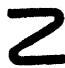
\includegraphics[keepaspectratio]{images/part002_406c0853.jpg}}

应当指出，若 \(f\) 是 \(\mathbf{Y}_1\) 到 \(\mathbf{Y}_2\) 上的双射且一致连续的映射，则它的连续延拓未必是单射，也未必是满射（习题 3）。
